\documentclass{article}
\usepackage{arxiv}
\usepackage[utf8]{inputenc}
\usepackage[T1]{fontenc}
\usepackage{hyperref}
\usepackage{url}
\usepackage{booktabs}
\usepackage{amsmath}
\usepackage{amssymb}
\usepackage{graphicx}
\usepackage{natbib}
\usepackage{xcolor}
\usepackage{microtype}

\graphicspath{{figures/}}
\hypersetup{colorlinks=true, linkcolor=blue!55!black, citecolor=blue!45!black, urlcolor=blue!55!black}
\bibliographystyle{plainnat}

\title{Essaymaster: Keeping a Research Paper Inside the Repository It Describes}
\author{Eyal Toledano\\ \texttt{eyal@tryhamster.com}}
\date{\today}
\preprintlabel{Essaymaster: Preprint}

\newcommand{\todo}[1]{\textcolor{red}{[\textbf{TODO:} #1]}}

% Match the output PDF version to the embedded vector figures (rsvg-convert emits
% PDF 1.7), silencing the xdvipdfmx version note.
\special{pdf:majorversion 1}
\special{pdf:minorversion 7}

\begin{document}
\maketitle

\begin{abstract}
A research paper about an actively developed system is the fastest-rotting document in
software: every landed optimization invalidates a number, every redesign invalidates a
claim, and unlike ordinary documentation a paper asserts measurements with its
author's credibility attached. We describe \textbf{essaymaster}, a discipline and an
accompanying agent toolkit for \emph{repo-resident} papers. The paper lives in the
repository it describes; every number it states flows through a provenance-tagged data
pipeline that admits exactly two states (sourced, or loudly flagged \texttt{TODO});
and an agent-run maintenance loop detects drift between the paper and the codebase,
then folds landed work back into the text.

The discipline was not designed on a whiteboard; it was extracted from five months of
practice maintaining the paper of a WebGPU inference engine. We mine that history as a
case study: 41 paper-maintenance commits (2026-03 to 2026-08) tracking a codebase that
moved by up to 117 commits between paper syncs; a provenance ledger that grew from 258
to 498 rows while its unsourced-row count fell from 16 to 8; review
passes whose numbered findings are reconstructible from commit messages; and a
one-command, network-free rebuild (data\,$\rightarrow$\,figures\,$\rightarrow$\,PDF)
measured at under five seconds, cheap enough to run on every sync. We report what the
discipline guarantees structurally, what it merely encourages, and what a single
self-reported case study cannot establish. This paper is itself the first end-to-end
run of the packaged pipeline; we present that as a demonstration, not as evidence.
\end{abstract}

\section{Introduction}
\label{sec:intro}

Research papers about living systems occupy an uncomfortable position. They are
written like publications, with fixed claims, fixed numbers, and a citation graph, but
they describe artifacts that change weekly. The conventional resolutions are all
unsatisfying: freeze the paper at submission time and let it drift into fiction;
rewrite it wholesale at each milestone and lose the audit trail; or never write it at
all, leaving the system's strongest results buried in commit messages and benchmark
logs. Software engineering has long known that ordinary documentation rots;
Lethbridge et al.\ found engineers reporting that documentation is usually not updated
after code changes~\citep{lethbridge2003documentation}, and \citet{olah2017research}
argue that un-distilled research accumulates a debt of its own. A numbers-bearing
systems paper is the worst case of both: it rots like documentation, but its rot is
\emph{falsehood} rather than staleness.

Essaymaster is a response built around one structural decision: \textbf{the paper is a
directory inside the repository it describes}, with the same standing as the code. It
is versioned with the code, built by it, reviewed in its pull requests, and updated at
the cadence of the work it reports. Around that decision we impose two invariants and
one maintenance contract:

\begin{itemize}
  \item \textbf{Invariant 1 (provenance-or-TODO).} Every number in the paper flows
  from a single curated data file in which each entry carries a provenance string (the
  file, log, or command it came from, with a date), through a deterministic
  consolidation script, into the tables and generated figures. A number the authors do
  not have is entered as the literal value \texttt{TODO}, propagates to a flagged row
  in the audit CSV, and renders in the PDF as a loud red marker. There is no third
  state, and there is no path by which a number enters the text directly.
  \item \textbf{Invariant 2 (structural honesty).} Unrun measurements are declared
  unrun in the paper itself, in the abstract and limitations rather than a footnote,
  and each one gets a committed runbook precise enough that a future session can
  execute it without re-deriving the design. Negative results are reported with their
  numbers. Replacing a headline number requires equal-or-better measurement rigor
  than the number it replaces.
  \item \textbf{The sync contract.} A small state file (\texttt{SYNC.json}) records
  the last repository commit the paper has absorbed and the paths whose changes could
  affect its claims. Drift is therefore a mechanical quantity, the count of watched
  commits since the last sync, computable by a shell script cheap enough to run at
  every agent-session start. Maintenance becomes a classification task over that
  commit range: changed number, new evidence, narrative shift, retraction trigger, or
  irrelevant.
\end{itemize}

The discipline is executed primarily by a coding agent. Essaymaster packages it as an
agent skill (a procedure document plus nine reference files encoding the rules
above), together with scaffold templates, miner and reviewer subagents, and two
drift-detection hooks, for the Claude Code harness~\citep{claudecode}. We view this packaging
through the lens of agent--computer interfaces~\citep{yang2024sweagent}: just as
agents resolve issues better when the repository is presented through an interface
designed for them~\citep{jimenez2024swebench}, an agent maintains a paper reliably
only when the paper's invariants are expressed as an explicit, checkable contract
rather than as good intentions.

This paper makes four contributions:
\begin{itemize}
  \item A \textbf{design} for repo-resident papers: the directory contract, the
  provenance-or-TODO number pipeline, the structural-honesty devices, and the
  \texttt{SYNC.json} drift mechanism (\S\ref{sec:design}).
  \item An \textbf{agent harness} for the design: the skill-and-references encoding,
  scaffolding templates with a deterministic offline build, and adversarial review
  with numbered findings (\S\ref{sec:harness}).
  \item A \textbf{five-month case study} mined from the git history of the practice
  the tool was extracted from, the Gerbil WebGPU engine paper~\citep{gerbil},
  quantifying maintenance cadence, drift between syncs, provenance-ledger growth, and
  the TODO burn-down (\S\ref{sec:casestudy}).
  \item An honest account of the \textbf{meta-circular demonstration}: this paper is
  the packaged pipeline's first end-to-end run, and we delimit exactly what that does
  and does not show (\S\ref{sec:meta}).
\end{itemize}

\section{The Problem: Papers Rot Faster Than Documentation}
\label{sec:problem}

Three properties make a systems paper harder to keep true than ordinary
documentation. First, \emph{claims are quantitative and perishable}: a README that
says ``fast'' survives an optimization campaign; a paper that says ``145 tokens/s''
does not. In the case study of \S\ref{sec:casestudy}, the flagship decode-throughput
figure was refreshed repeatedly across the LaTeX paper's seven-week lifetime, from
145 tokens/s in its first committed abstract to a 347.3 tokens/s kept peak in its
last refresh (2.4$\times$). Each refresh was a statement the old text had silently
stopped being true.
Second, \emph{drift is bursty}: repositories move in campaigns. Between two adjacent
paper-maintenance commits in our corpus, up to 117 non-paper commits landed in a
16-day window. A paper synchronized weekly by habit would have been badly wrong
mid-window and needlessly touched in quiet weeks; drift needs to be measured, not
scheduled.
Third, \emph{the failure mode is silent}: nothing breaks when a paper claim goes
stale. Code has tests; papers have only their authors' memory. The essaymaster
position is that this third property is the one worth engineering away. Staleness
must be made \emph{visible} (a drift count printed at session start, and a nudge in
the commit output at the moment landed work touches watched paths) and falsehood
made \emph{structurally difficult} (no unsourced number can enter the text
unflagged).

\section{Design: The Paper as a Repository Contract}
\label{sec:design}

\subsection{The directory contract}
A paper under essaymaster is a self-contained directory (\texttt{paper/}, or
\texttt{papers/$\langle$slug$\rangle$/} once a repository hosts several) holding the
LaTeX source, a verified bibliography, the curated data file, two zero-dependency
generator scripts (consolidation and figures), a one-command build, and the sync
state. The contract is that the directory builds from a bare checkout with no GPU and
no network. Anyone can regenerate every table, figure, and page from the committed
data: continuous integration, a teammate, or an agent deciding whether its own edit
broke something.

\subsection{Invariant 1: the number pipeline}
\label{sec:pipeline}
All measured values live in one curated JSON file in which every block carries a
provenance string. A consolidation script flattens it into an audit CSV
(\texttt{key, value, is\_todo, provenance}; one greppable row per number) and into
the per-figure data series; a figure script renders those series to SVG with no
external chart library. The LaTeX source cites numbers that exist in the ledger and
includes figures that were generated from it; hand-transcribing a number into the
text is a protocol violation that review is instructed to hunt for. The pipeline's
value is less automation than \emph{auditability}: ``where does this number come
from?'' is answered by one grep, for every number, forever.

\subsection{Invariant 2: structural honesty}
\label{sec:honesty}
Honesty devices that depend on author diligence decay under deadline pressure, so the
discipline makes them structural. The \texttt{TODO} state is first-class: it survives
consolidation, is counted by the build, and renders in red in the PDF, so an
unsourced number is never invisible. Pending measurements get a committed
\emph{ablation runbook} stating why each matters, the exact protocol, and the
instruction that no paper number may be filled from the runbook until the run has
actually executed. A \emph{reviewer-readiness checklist} maps every remaining gap to
its flagged rows, making ``submittable'' a checkable predicate rather than a feeling.
And replacement of a headline number demands equal-or-better rigor (same or more
runs, same protocol), so numbers ratchet toward reliability rather than toward
recency.

\subsection{The sync contract}
\label{sec:sync}
\texttt{SYNC.json} records \texttt{lastSyncedCommit} and \texttt{watchedPaths}. Drift
is \texttt{git log lastSyncedCommit..HEAD -- watchedPaths}, a number a hook can print
in one line at session start. A companion git post-commit hook closes the loop from
the other side: when a landed commit touches watched paths without touching the
paper, the committer (agent or human) is nudged in the commit output itself, so the
``does the paper need this?'' question is raised at the moment of landing rather
than at the next session. A sync is then a bounded editorial procedure: classify
each watched commit (changed number, new evidence for an existing claim, narrative
shift, retraction trigger, or irrelevant); apply changes \emph{through the data
pipeline first}, then the prose; rebuild; advance the sync pointer; commit per theme
with a \texttt{paper:} prefix so the maintenance history remains legible. Retraction
triggers, meaning landed work that falsifies a paper statement, outrank everything
else, on the principle that a stale overclaim is worse than any gap.

\section{The Agent Harness}
\label{sec:harness}

The discipline is executed by a coding agent, and the packaging reflects a specific
belief: for editorial work, the right agent interface is \emph{prose contracts plus
mechanical checks}, not end-to-end automation. The skill's procedure document routes
among seven modes (mine, mine-sessions, init, sync, build, review, publish); nine
reference files carry the rules of \S\ref{sec:design} in the imperative,
checklist-bearing form agents follow reliably. The mechanical parts are plain scripts: drift counting,
toolchain probing, consolidation, figure generation, the build. An agent should never
be trusted to \emph{compute} what a script can compute. The judgment parts remain
agent work bounded by the invariants: classifying a landed commit, deciding whether a
feature is a contribution, wording a qualifier.

The subagents divide by corpus. The \emph{miner} performs read-only archaeology over
the repository: given a slice, it extracts candidate paper material (optimization
campaigns with recorded numbers, non-obvious theses in design docs, negative
results), each find paired with a web-verified novelty check. The
\emph{session-miner} sweeps the agent's own session transcripts for the material git
structurally cannot show: measured dead ends that never reached a commit, multi-step
diagnosis arcs, and recurring cross-session patterns; its finds are treated as
lab-notebook leads that must be re-run or explicitly flagged before entering a
ledger, and only session-exclusive material survives the dedupe against git. The \emph{reviewer} is adversarial
and edit-free: it returns numbered findings across four lenses (evidence, drift,
citations, honesty), which are then fixed in commits referencing the finding ids, so
the review trail is reconstructible from history alone (\S\ref{sec:casestudy}
verifies this actually happens in practice). Citation hygiene is its own reference
file with one absolute rule: every citation is verified by web search in the session
that adds it, and systems without papers are cited as repositories, never as
invented arXiv ids.

Init deliberately front-loads planning. Before any LaTeX exists, the agent commits a
plan document containing the verified related-work survey, the genre choice, and a
\emph{claims-to-required-evidence table} whose rows are the only claims the paper is
permitted to make. The paper is then written evidence-first, evaluation skeleton
before introduction, so that an unwritable evaluation section is discovered on day
one rather than at submission.

\section{Case Study: Five Months of the Gerbil Paper}
\label{sec:casestudy}

The discipline was extracted from, not imposed on, the paper of the Gerbil WebGPU
inference engine~\citep{gerbil}: a $\sim$17-page arXiv-style systems preprint that
lives in that repository's \texttt{paper/} directory. We mined the practice
retrospectively on 2026-08-25 from the repository's git history using read-only
commands, each recorded alongside its number in this paper's own data ledger. Two
scope caveats apply throughout. First, the corpus of ``paper-maintenance commits'' is
every commit touching the paper directory, its engineering-reference precursor
document, or the two planning documents, on the current branch: 41 commits from
2026-03-11 to 2026-08-10. The earliest four (March) are engine feature commits that
updated the engineering reference as a side effect; the LaTeX paper proper begins
2026-06-23. Second, this is a single practice, mined by the people who ran it;
\S\ref{sec:limits} treats the resulting biases.

\begin{figure}[t]
  \centering
  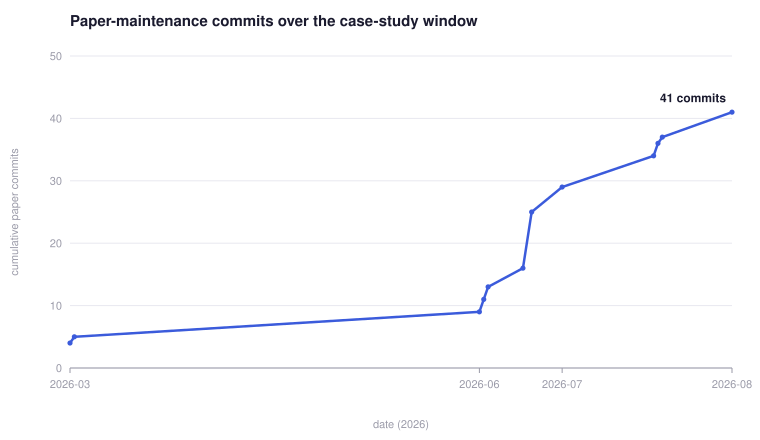
\includegraphics[width=0.85\linewidth]{fig1_commit_cadence}
  \caption{Cumulative paper-maintenance commits in the case-study repository
  (41 commits, 2026-03-11 to 2026-08-10, current-branch corpus). The staircase shape
  is the practice's signature: maintenance arrives in bursts on 12 distinct days,
  up to nine commits in a day, rather than on a schedule. The burst timing is
  consistent with campaign-driven maintenance (\S\ref{sec:problem}); the June
  cluster also includes the initial planning and drafting work.}
  \label{fig:cadence}
\end{figure}

\subsection{Cadence: syncs follow campaigns}
Figure~\ref{fig:cadence} shows the maintenance cadence. The paper was touched on just
12 distinct days across five months, in bursts of up to nine commits per day. This is
consistent with the design position (\S\ref{sec:problem}) that paper maintenance
should track campaign boundaries, not calendars. Table~\ref{tab:synclag} quantifies
the drift those bursts absorbed: between adjacent paper commits, the repository moved
by anywhere from zero to 117 non-paper commits. The measure is an upper bound, since
a commit touching both code and paper counts as non-paper, but the shape is the
point: drift arrives in avalanches, and a mechanism that \emph{measures} it (the
\texttt{SYNC.json} count) dominates one that assumes a rate.

\begin{table}[t]
  \centering
  \small
  \begin{tabular}{llrr}
    \toprule
    Sync commit (date) & Previous sync & Commits between & \ldots non-paper \\
    \midrule
    2026-08-10 & 2026-07-25 & 120 & 117 \\
    2026-07-25 & 2026-07-24 & 14 & 14 \\
    2026-07-24 & 2026-07-23 & 30 & 29 \\
    2026-07-23 & 2026-07-02 & 38 & 33 \\
    2026-07-02 & 2026-07-02 & 15 & 11 \\
    \bottomrule
  \end{tabular}
  \caption{Repository movement between selected adjacent paper-maintenance commits
  (the five largest gaps among the fifteen most recent pairs). ``Non-paper'' counts
  commits whose diff touches any watched non-paper path and is an upper bound on
  drift, since mixed commits count as non-paper.}
  \label{tab:synclag}
\end{table}

\subsection{The provenance ledger: growth with a shrinking gap list}
Figure~\ref{fig:burndown} tracks the audit CSV across its eight committed versions.
The ledger nearly doubled, from 258 to 498 total rows, while the count of
\texttt{TODO}-flagged rows among them fell from 16 to 8 (peaking at 18 as an honest
sweep added new known-unknowns before closing them); fully sourced rows thus grew
from 242 to 490. The residual 8 are not debt hidden in the
text: each maps to a declared pending measurement in the repository's committed
runbook, and four render as visible red markers in the shipped PDF. This is the
intended equilibrium of Invariant 2. The gap list shrinks, but more importantly it is
\emph{enumerable} at every point in history by a single grep over a committed file.

\begin{figure}[t]
  \centering
  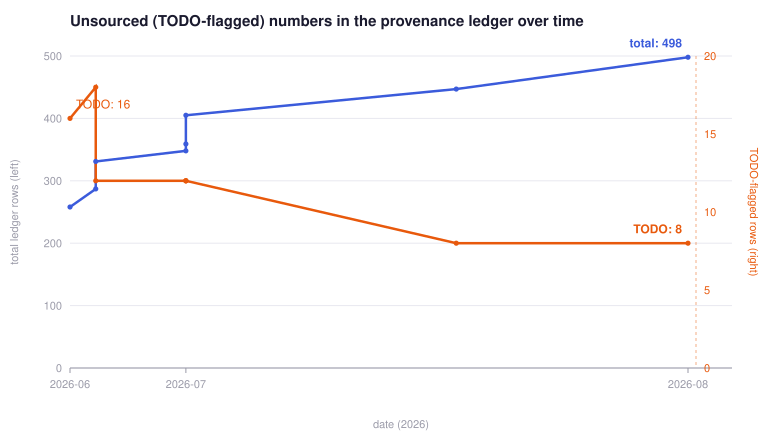
\includegraphics[width=0.85\linewidth]{fig2_todo_burndown}
  \caption{The provenance ledger over its eight committed versions: total rows
  (blue, left axis) versus the \texttt{TODO}-flagged subset (orange, right axis).
  Rows were added at roughly 150 per month over the ledger's seven-week lifetime
  while the unsourced subset halved; the transient rise to 18 is a sweep that added
  new known-unknowns before closing them.}
  \label{fig:burndown}
\end{figure}

\subsection{Review passes leave a reconstructible trail}
Four commits in the corpus carry review evidence, three of them referencing numbered
findings in their subjects, e.g.\ \emph{``qualify causal claim in
abstract+contributions (review \#E1/E3/E4)''} and a reframing commit closing findings
\#E1--E7 and \#D1--D2. The finding taxonomy observed in the wild used evidence (\#E),
drift (\#D), and abstract-level (\#A) lenses; the citation (\#C) and honesty (\#H)
lenses the packaged reviewer now carries never appear in the historical log. The
packaged tool extends the observed practice there, and we flag that as codification
rather than extraction. The substantive point survives the caveat: the practice's
strongest single honesty event, weakening a causal claim in its own abstract, is a
one-line commit anyone can find.

\subsection{The build is cheap enough to be unskippable}
The case-study paper rebuilds in 4.7 seconds of wall clock on the authoring machine
(single run, warm engine cache; indicative, not a benchmark). That rebuild covers a
498-row consolidation, corpus cleaning that logs what it \emph{dropped} (29
adversarial rows, an instance of the no-silent-caps rule), nine SVG figures,
vector conversion, and a 17-page PDF via tectonic~\citep{tectonic}. The number
matters only relative to a threshold: rebuild cost this low removes the last excuse
for committing an unbuilt paper, so ``the PDF in the repo is the current claims''
stays true. Snapshot totals at mining time: 498 ledger rows (8 flagged unsourced),
51 verified bibliography entries, 1{,}365 lines of LaTeX, 9 generated figures, 17
pages.

\section{The Meta-Circular Demonstration}
\label{sec:meta}
This paper was produced as the packaged pipeline's first end-to-end run: a miner
subagent extracted every case-study number above from the Gerbil history; seven
external citations were web-verified in the authoring session; the paper directory
was scaffolded from the shipped templates; the two figures were generated by the
zero-dependency pipeline from the provenance ledger (118 rows, 0 flagged); and the
PDF builds offline by the standard one-command path. We state plainly what this
shows and does not. It demonstrates the pipeline is \emph{executable} end-to-end by
an agent, including its verification steps. It is not evidence the discipline
improves outcomes, both because a demonstration chosen by the tool's authors proves
availability rather than benefit, and because the case study it reports predates the
packaging. The packaged tool's own five-month history does not exist yet; when it
does, it will be minable by exactly the procedure of \S\ref{sec:casestudy}.

\section{Related Work}
\label{sec:related}
\textbf{Documents that live with code.} Literate programming made the program and its
explanation one artifact~\citep{knuth1984literate}; computational notebooks made the
analysis document executable~\citep{kluyver2016jupyter}. Essaymaster inverts the
first (the \emph{paper} moves in with the code, keeping its publication genre) and
complements the second (the executable part is the pipeline \emph{around} a static
PDF, because arXiv-genre papers, not notebooks, are the target artifact). The
docs-as-code practice community applies versioning and CI to documentation broadly;
essaymaster is that stance specialized to the document class with the strictest
truth obligations. \citet{olah2017research} name the debt;
\citet{lethbridge2003documentation} measured the rot for ordinary documentation two
decades ago.
\textbf{Agents in repositories.} SWE-bench established repository-level issue
resolution as an agent task~\citep{jimenez2024swebench}, and SWE-agent showed the
interface presented to the agent dominates outcomes~\citep{yang2024sweagent};
essaymaster's skill-plus-invariants packaging is an agent--computer interface for
editorial maintenance rather than code change.
\textbf{Agent-written papers.} The AI Scientist automates the full
idea-to-manuscript loop~\citep{lu2024aiscientist}. Essaymaster occupies the opposite
corner deliberately: papers whose claims are owned by humans and grounded in a
repository's recorded measurements, where the agent's autonomy is spent on
\emph{maintenance and verification}, the part humans demonstrably neglect, rather
than on generation. We found no published treatment of this maintenance problem
(keeping a long-lived paper continuously consistent with a moving codebase under
machine-checkable provenance) and state that gap as this paper's niche, with the
survey-breadth caveat of \S\ref{sec:limits}.

\section{Limitations}
\label{sec:limits}
The evaluation is a single case study ($n{=}1$), of a practice run by this paper's
author, mined and written up with the tool being described: three concentric
conflicts we mitigate with recorded extraction commands and stated caveats, not
eliminate. The case study validates the \emph{discipline} (it was really followed,
for five months, at low cost); it cannot validate the \emph{packaged tool}, which
post-dates it, nor compare against ad-hoc maintenance by other teams. The controlled
study essaymaster's own methodology would demand is future work, and Claim~6 of our
plan's claims table is accordingly marked not-claimable. The drift measure is an
upper bound; the build timing is a single warm-cache run; the review-lens taxonomy
partially post-dates the evidence for it; and the related-work search, while
verified entry-by-entry, was breadth-limited. Adjacent literatures (scientific
workflow provenance, artifact evaluation, living reviews) may hold closer neighbors
than we found.

\section{Conclusion}
\label{sec:conclusion}
A paper that lives with its codebase can stay true the way code stays working: by
making its freshness measurable, its numbers auditable, and its gaps loud. Five
months of one practice suggest the cost is modest (twelve days of touches, a
five-second rebuild), and the packaged form makes the discipline transferable to
any repository with an agent attached. Whether it transfers \emph{well} is now an
empirical question the tool is instrumented to answer about itself.

\bibliography{refs}

\appendix
\section{Artifact Appendix}
\label{sec:artifact}
Essaymaster (skill, references, commands, agents, hook, scripts, templates, and this
paper's full source and data) is the repository this paper resides
in~\citep{essaymaster}; the repository is private at the time of writing, with public
release planned alongside any public posting of this paper. Rebuild: \texttt{cd paper \&\& ./build.sh} (requires Node;
the PDF step requires tectonic or a TeX Live engine; figures use rsvg-convert when
present). Every case-study number is a row in \texttt{results/measurements.csv}
whose provenance field records the exact extraction command; the mining was performed
against \texttt{github.com/tryhamster/gerbil} at branch \texttt{docs/paper-two-column}
on 2026-08-25. The paper class is the MIT-licensed \texttt{arxiv.sty} derivative
shipped with the templates~\citep{arxivstyle}.

\end{document}
